\documentclass[aspectratio=169]{beamer}
\usetheme{Bruno}
\usepackage{amsmath}
\usepackage{amssymb}
\usepackage{siunitx}
\usepackage{float}
\usepackage{tikz}
\def\checkmark{\tikz\fill[scale=0.4](0,.35) -- (.25,0) -- (1,.7) -- (.25,.15) -- cycle;} 
\usepackage{url}
\usepackage[siunitx,american,RPvoltages]{circuitikz}
\ctikzset{capacitors/scale=0.7}
\ctikzset{diodes/scale=0.7}
\usepackage{tabularx}
\newcolumntype{C}{>{\centering\arraybackslash}X}
\renewcommand\tabularxcolumn[1]{m{#1}}% for vertical centering text in X column
\usepackage{tabu}
\usepackage[spanish,es-tabla,activeacute]{babel}
\usepackage{babelbib}
\usepackage{booktabs}
\usepackage{pgfplots}
\usepackage{hyperref}
\hypersetup{colorlinks = true,
            linkcolor = black,
            urlcolor  = blue,
            citecolor = blue,
            anchorcolor = blue}
\usepgfplotslibrary{units, fillbetween} 
\pgfplotsset{compat=1.16}
\usepackage{bm}
\usetikzlibrary{arrows, arrows.meta, shapes, 3d, perspective, positioning,mindmap,trees,backgrounds}
\renewcommand{\sin}{\sen} %change from sin to sen
\usepackage{bohr}
\setbohr{distribution-method = quantum,insert-missing = true}
\usepackage{elements}
\usepackage{verbatim}
\usepackage[edges]{forest}
\usepackage{etoolbox}
\usepackage{schemata}
\usepackage{appendix}
\usepackage{listings}

\definecolor{color_mate}{RGB}{255,255,128}
\definecolor{color_plas}{RGB}{255,128,255}
\definecolor{color_text}{RGB}{128,255,255}
\definecolor{color_petr}{RGB}{255,192,192}
\definecolor{color_made}{RGB}{192,255,192}
\definecolor{color_meta}{RGB}{192,192,255}
\newcommand\diagram[2]{\schema{\schemabox{#1}}{\schemabox{#2}}}

\definecolor{codegreen}{rgb}{0,0.6,0}
\definecolor{codegray}{rgb}{0.5,0.5,0.5}
\definecolor{codepurple}{rgb}{0.58,0,0.82}
\definecolor{backcolour}{rgb}{0.95,0.95,0.92}

\lstdefinestyle{mystyle}{
    backgroundcolor=\color{backcolour},   
    commentstyle=\color{codegreen},
    keywordstyle=\color{magenta},
    numberstyle=\tiny\color{codegray},
    stringstyle=\color{codepurple},
    basicstyle=\ttfamily\footnotesize,
    breakatwhitespace=false,         
    breaklines=true,                 
    captionpos=b,                    
    keepspaces=true,                 
    numbers=left,                    
    numbersep=5pt,                  
    showspaces=false,                
    showstringspaces=false,
    showtabs=false,                  
    tabsize=2
}

\lstset{style=mystyle}
\title{Instrumentación I: \\ \emph{Introducción a la }\\ \emph{instrumentación industrial.} \\ \emph{Primera sesión}}
\author{
    Juan J. Rojas, Hugo Sanchez Ortiz
}
\institute{Instituto Tecnológico de Costa Rica}
\date{\today}
\background{fig/background.jpg}
\begin{document}
\sisetup{unit-math-rm=\mathrm,math-rm=\mathrm} % change sinitx font
\sisetup{output-decimal-marker = {,}}
\maketitle

\newcommand{\blackandwhite}{white} %change this at the end

\begin{frame}[t]{Sistemas embebidos}
Es un computador diseñado para realizar alguna función especifica dentro de un sistema complejo. Típicamente opera sin intervención del usuario a diferencia de un computador personal.  

\begin{tikzpicture}[remember picture, overlay]
    \node[above=0.5cm] at (current page.south) 
    {
        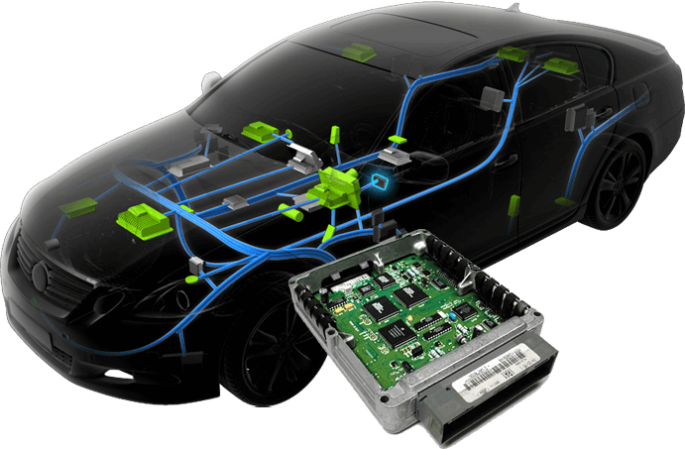
\includegraphics[width=0.55\textwidth]{fig/embebidos.png}
    };
\end{tikzpicture}
\end{frame}

\begin{frame}[t]{Microcontroladores}
Son circuitos integrados compactos diseñados para gobernar alguna operación especifica en un sistema embebido. Incluyen un procesador, memoria (RAM y ROM/flash) y periféricos de entrada/salida en un solo chip.

\begin{tikzpicture}[remember picture, overlay]
    \node[above=0.5cm] at (current page.south) 
    {
        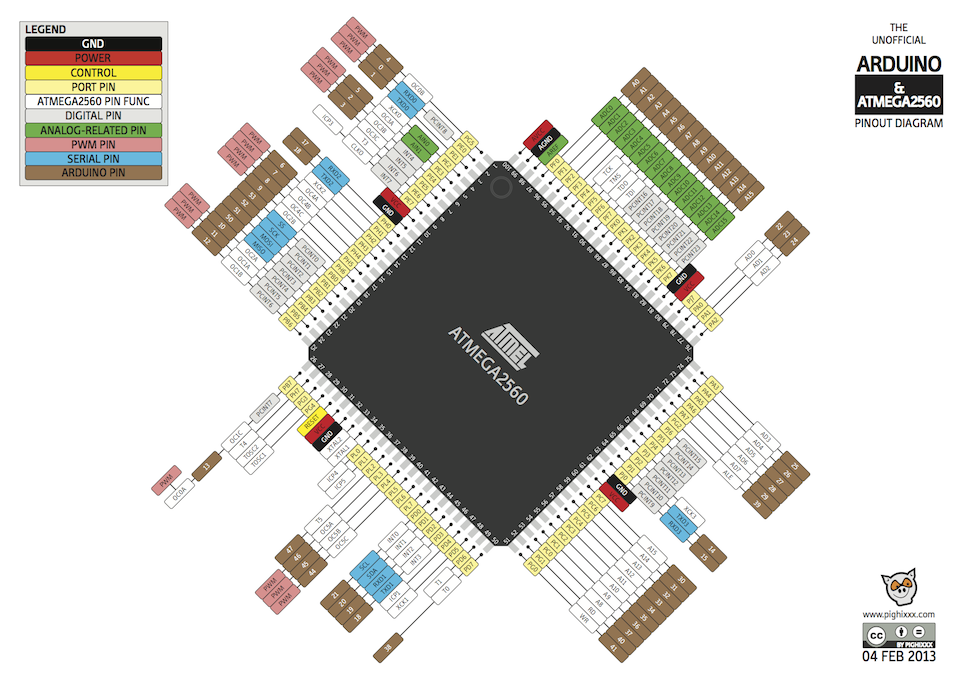
\includegraphics[width=0.5\textwidth]{fig/ATMEGA2560.png}
    };
\end{tikzpicture}
\end{frame}

\begin{frame}[t]{Placas de desarrollo}
Son plataformas de hardware diseñadas para ayudar a crear y validar aplicaciones de sistemas embebidos. Estas placas generalmente incluyen un microcontrolador o microprocesador, junto con una serie de periféricos y conectores que facilitan la conexión de sensores, actuadores, y otros componentes necesarios para el desarrollo de un proyecto embebido.

\begin{tikzpicture}[remember picture, overlay]
    \node[above=0.5cm] at (current page.south) 
    {
        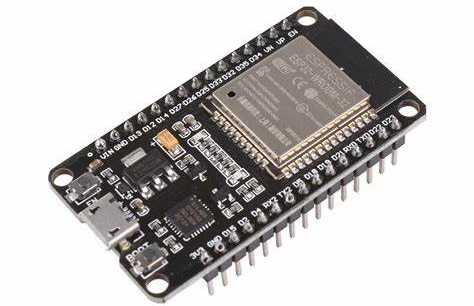
\includegraphics[width=0.5\textwidth]{fig/ESP32.jpeg}
    };
\end{tikzpicture}
\end{frame}



\begin{frame}[t]{Lenguajes de programación: niveles}
El nivel de un lenguaje de programación se define según su relación con el lenguaje humano. Un lenguaje de programación de alto nivel es uno que está mas cerca de los lenguajes humanos y mas lejos del lenguaje de máquina

\begin{tikzpicture}[remember picture, overlay]
    \node[above] at (current page.south) 
    {
        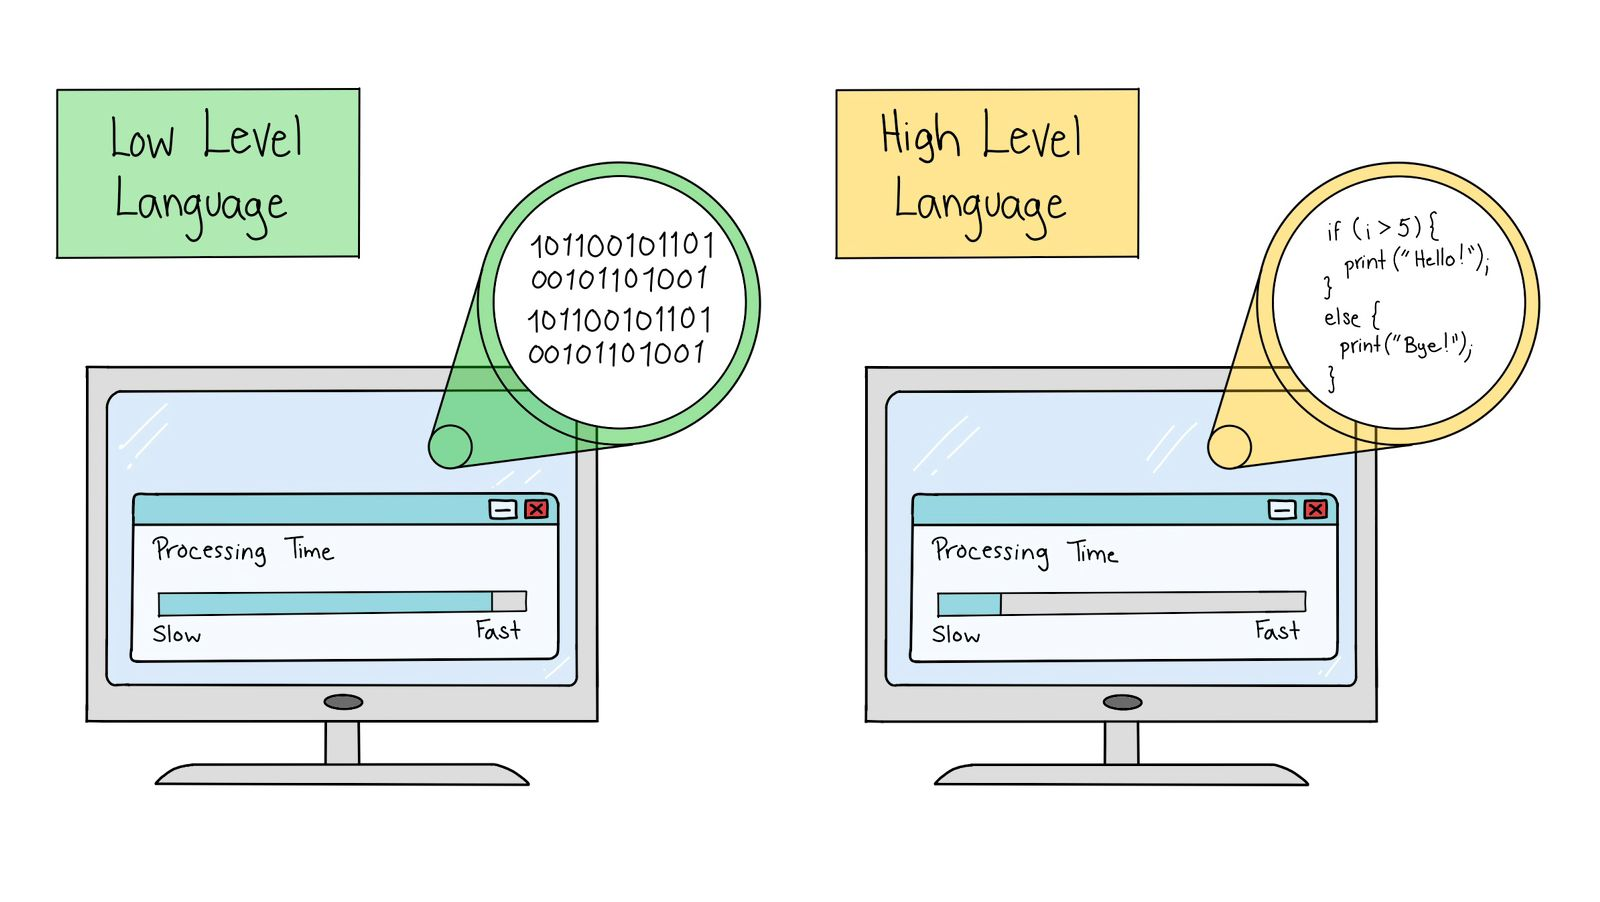
\includegraphics[width=0.7\textwidth]{fig/niveles.jpg}
    };
\end{tikzpicture}
\end{frame}

\begin{frame}[t]{Lenguajes de programación: compilado o interpretado}

\begin{tikzpicture}[remember picture, overlay]
    \node[above] at (current page.south) 
    {
        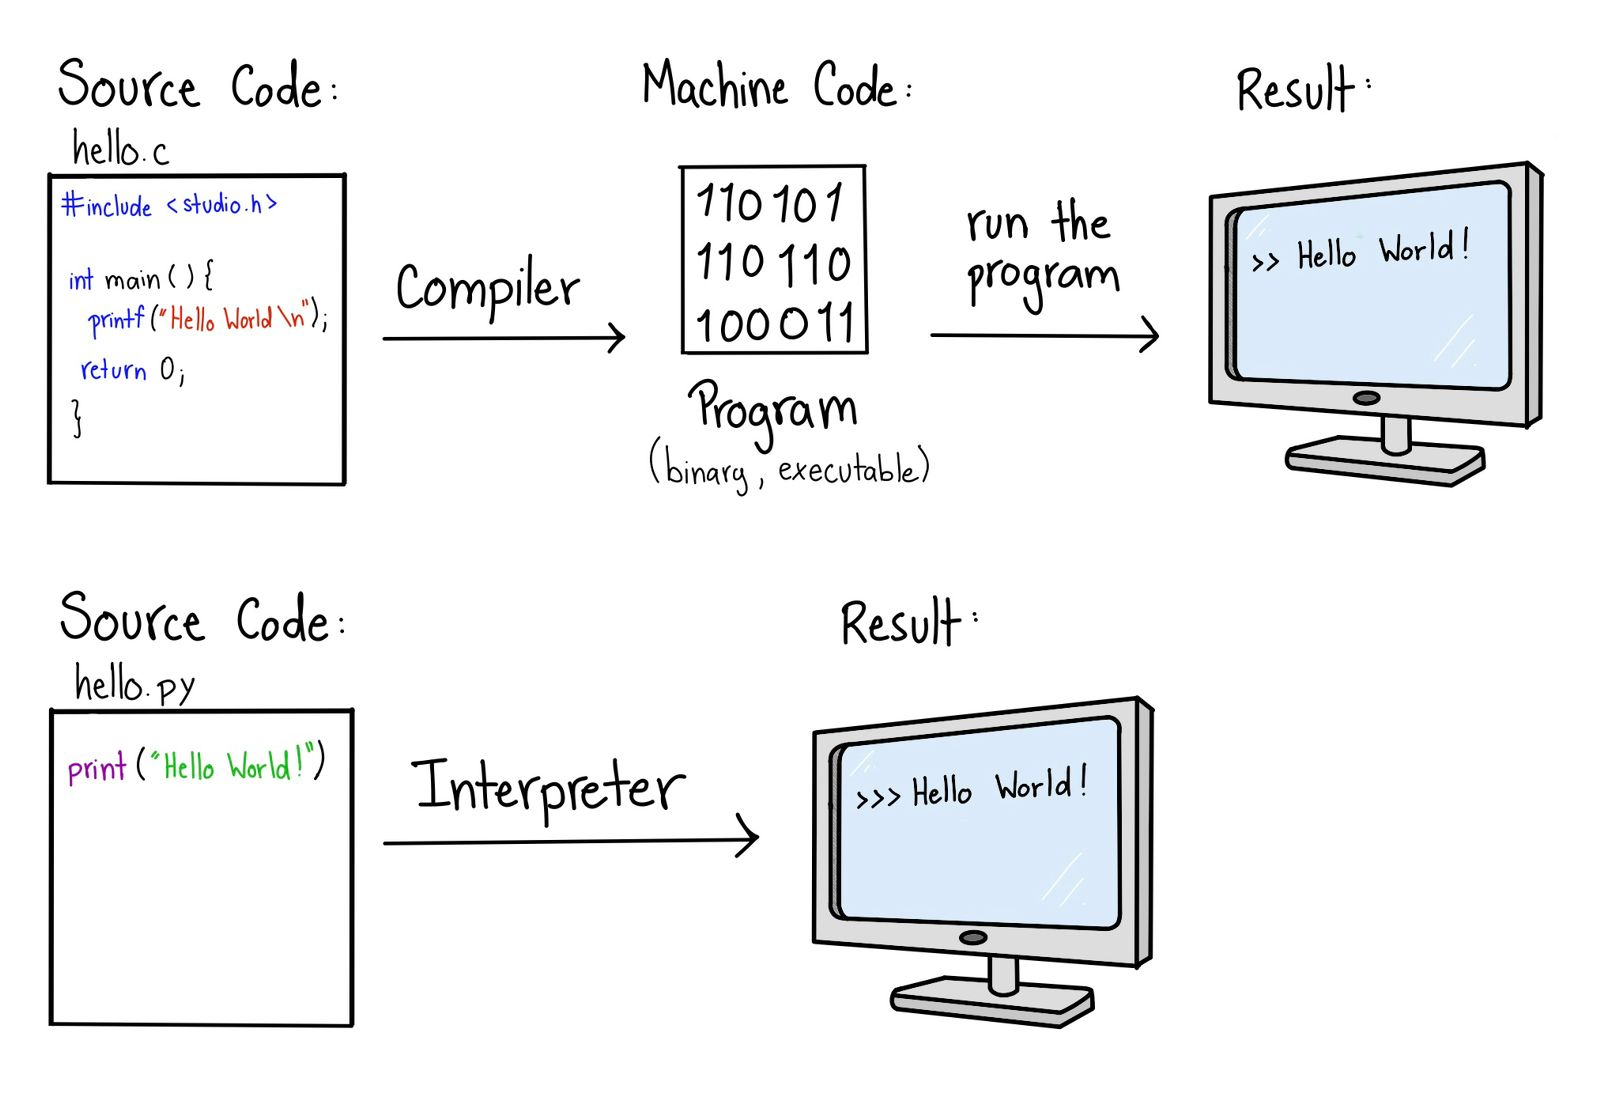
\includegraphics[width=0.75\textwidth]{fig/compiladovrsinterpretado.jpg}
    };
\end{tikzpicture}
\end{frame}

\begin{frame}[t]{C y C++}
\begin{itemize}
    \item \textbf{C} es un lenguaje de programación de propósito general, de bajo nivel, desarrollado a principios de la década de 1970 por Dennis Ritchie en los Laboratorios Bell de AT\&T. C fue creado inicialmente para desarrollar el sistema operativo Unix, y desde entonces se ha convertido en uno de los lenguajes de programación más influyentes y utilizados en la historia de la informática.
    \item \textbf{C++} es una extensión del lenguaje C, desarrollada por Bjarne Stroustrup en los años 1980. C++ se diseñó para añadir características orientadas a objetos a C, lo que lo convierte en un lenguaje híbrido que soporta tanto programación orientada a objetos como programación procedimental.
\end{itemize}
\end{frame}

\begin{frame}[t]{Variables y tipos}
\begin{itemize}
    \item \textbf{Variable} identifica una ubicación en la memoria del computador en la que puede guardar datos que pueden ser modificados durante la ejecución del programa.
    \item \textbf{Tipos de datos} define que tipo de valor y que operaciones se pueden realizar con una variable específica 
\end{itemize}
\end{frame}

\begin{frame}[t]{Tipos de datos numéricos en C y C++}
\begin{columns}[c, onlytextwidth]
    \begin{column}{0.5\textwidth}
        Tipos: 
        \begin{itemize}
            \item \textbf{int}
            \item \textbf{char}
            \item \textbf{float}
            \item \textbf{double}
            \item \textbf{void}    
        \end{itemize}
        Modificadores
        \begin{itemize}
            \item \textbf{signed}
            \item \textbf{unsigned}
            \item \textbf{short}
            \item \textbf{long}  
        \end{itemize}
    \end{column}
    \begin{column}{0.5\textwidth}
        Derivados: 
        \begin{itemize}
            \item \textbf{array}
            \item \textbf{pointer}
            \item \textbf{struct}
            \item \textbf{union}
            \item \textbf{enum}    
        \end{itemize}
        C++
        \begin{itemize}
            \item \textbf{bool}
            \item \textbf{wchar\_t}
            \item \textbf{string}
            \item \textbf{class}  
        \end{itemize}
    \end{column}
\end{columns}

\end{frame}

% \begin{frame}{Referencias}

% \bibliographystyle{ieeetr}
% \footnotesize
% \bibliography{comunes/referencias}

%\end{frame}

\end{document}